\documentclass{article}
\usepackage{a4wide}
\usepackage{graphicx}

\title{Assignment 3}
\begin{document}
\author{Cupak Miroslav,\\
		Nizan Juraj, \\
        Nemecek David,\\
		Streck Adam}
\maketitle

\section{Concept}
We want to build a robot capable of:
\begin {enumerate}
\item Calibrating its track and light detection sensor.
\item Reading instructions in some graphical represenatation while riding over them.
\item Visible execution of those instructions.
\end {enumerate}

\section{Design}

\subsection{Behaviour}
There are four basic things such a robot could do:
\begin{enumerate}
\item Move and steer.
\item Make sounds.
\item Draw on LCD of the NTX brick.
\item Use third motor to do something.
\end{enumerate}
I would pick two of them - move and make sounds, unless movement is too loud for sound to be audible, I will fruthemore explain how to utilize them.

\subsection{Construction}
What sort of the hardware we use? How did you design it? What probles you have encountered while building it?

For self-calibration of the position is best to use three wheel vehicle with signe free wheel in the front and two wheels with independent motors in the back (sort of the thing that is built right now). \\
However, I think that 4-wheel vehicle with single motor for movement and second one for steering will be better for execution of instructions and overall more awesome, so I suggest building that one - there is a howto for one pretty, I would build on that: \verb+http://www.nxtprograms.com/NXT2/race_car/steps.html+ .

\subsection{Movement programming}
How the movement routine looks? What is it capable of?

\subsection{Light calibraion}
How do you calibrate light sensors?

\section{Coding}

\subsection{Code representation}
How do you encode instructions? What are adventeges and disadvanteges of this representations? How is it read? Do you use some special symbols?

I see two ways how to make coding (I already nicknamed the language \emph{GreyDot}, do you agree?):
\begin{itemize}
\item Use scale for gray with 10 steps.
\item Use triples of black (0) and gray (1).
\end{itemize}
First option would be better, but we need to test if we can always calibrate the sensor so it reads correct instructions no matter what light conditions are - but it should work, when I tested it, it was pretty sharp. In this case we have 9 steps for different instructions and 1 for background. \\
Second option uses only three steps - black for 0, grey for 1 and white for background and I am pretty positive that this option would work even without self calibration. We would than have 8 combinations.

\subsection{Special symbols}
There is at leas one symbol left for each line - these will be used as special symbols - for now we may need these symbols:
\begin{enumerate}
\item maybe - Start color calibration (should be black-black).
\item maybe - Start path calibration.
\item sure - Start reading instructions.
\item sure - End reading instructions and execute.
\end{enumerate}

\subsection{Writing instructions}
How do you write instruction files? How do you plot them?

I would write instructions in simple ASCII file and then have some script plot it. \\
I would recomment using two lines - first for movement with numbers of instructions of some symbolic representation - < for steer left etc. \\



\subsection{Movement calibration}
How do you ensure robot stays on the path and reads instructions? How do you cope with errors?

\subsection{Reading data}
Although in the beginning it seemed as a simple task, reading the data
from the data-line turned out to be quite tricky. One would expect that
when the light sensor moves from a white region onto a black region,
it would result in a few readings of WHITE and then BLACK values. Instead
it results in WHITE - GREY - DARK GREY - BLACK values.

\subsubsection{Data encoding}
Because the light sensor is basically an analog input device, the outgoing
values have to be treated that way - as an analog signal. And as the device
is not that sensitive, we decided (for the sake of reliability) to reduce
the number of recognized colors to three: WHITE, GREY, BLACK.

This gives us the option to encode binary strings into a 3-level signal.
WHITE being the \textit{no-data}, \textit{synchronization} level and GREY
and BLACK being the \textit{data} levels, 0 and 1 respectively. Every
signal interval between two WHITE regions is considered to be one bit and
based on the maximal value (darkness of the color) we recognize its value.

This is a "peak value encoding" with automatic synchronization.
The encoding therefore delivers 1 bit of information for every two signal
elements (changes).

\begin{figure}[h]
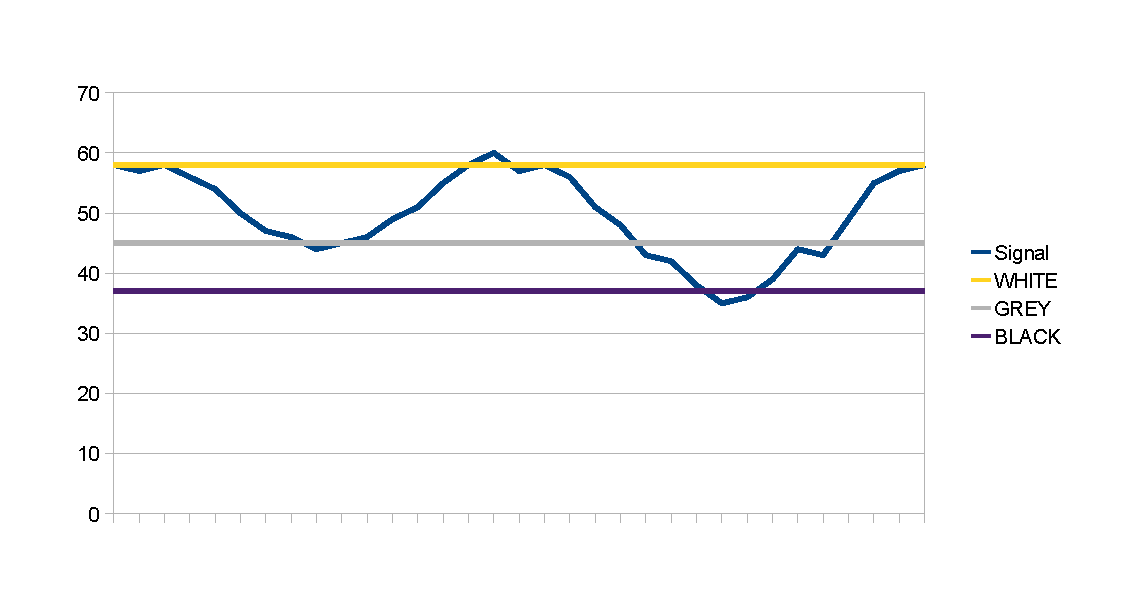
\includegraphics[width=1.0\linewidth]{light_signal.pdf}
\caption{Light sensor readings}
\end{figure}

\subsubsection{Various details}
After testing a few layouts and configurations we found that the best
results are achieved with \textit{data} stripes 2~cm thick and
\textit{synchronization} spaces about 3~cm thick. Thin stripes
tend to be overlooked by the robot, extra thick \textit{data} stripes
could be erroneously interpreted as multiple bits. Larger areas of white
do not matter much, although there is always the possibility of picking
up "noise" bits (e.g. dirt marks).

The cooperation of the line-following (main) and data-reading (slave) threads
proved to be essential. When the robot leaves the guiding line, it needs
to stop, adjust its direction and then continue again.
This often results in erroneously read or re-read bits, because the
data-line is not moving strictly in one direction. The master thread
therefore signals the slave thread when it is safe to read data values
(i.e. the robot is moving forward).

\subsubsection{Error handling}
To make the encoding as simple as possible, we implemented a
timeout-based reading termination to avoid control sequences in the data
flow. Every successfully read bit resets the timer, otherwise after
a specified timeout the reading process is terminated. This signals
the main line-following thread that it should terminate as well.

In the end the resulting array of bits is converted into an array of
2-bit \textit{bytes}. This implies an even number of bits, which is the
only error-checking performed by the decoder. Bit values are not checked
in any way as it would require more bits to be read.



\section{Instructions execution}
The final phase of the robot's program aims to interpret the newly decoded
binary data. This works as expected: the instruction interpreter sets its
Program Counter (PC) to the first data \textit{byte} (i.e. 2-bit value)
which determines what should be executed and then repeats the whole
process until it moves out of the array of instructions. Every
instruction moves the PC one \textit{byte} further, instructions have
access to the PC and can (theoretically) alter it to perform loops.

\subsection{Instruction set}
Although it would be possible to prepare a "Turing-complete" set
of instructions, our goal was to showcase that the robot does what it is
told using only a few bytes.
The same goes for the number of instructions - we used 2-\textit{byte}
instructions (first its function, then its parameter), but it is
possible to have longer / shorter / variable length instructions.

\begin{center}
\begin{tabular}{|c|c||l|}
\hline
\textbf{Byte 1}   &   \textbf{Byte 2}   &   \textbf{Description}\\
\hline
\hline
    0   &   0       &   Go forward\\
        &   1       &   Go forward left\\
        &   2       &   Go forward right\\
        &   3       &   Repeat LAI 2x\\
\hline
    1   &   0       &   Go back\\
        &   1       &   Go back left\\
        &   2       &   Go back right\\
        &   3       &   Repeat LAI 5x\\
\hline
    2   &   X       &   Play tone (X+1) * 100~Hz\\
\hline
    3   &   X       &   Delay time (X+1) * 1000~ms\\
 \hline
 \end{tabular}
\end{center}

Every standard instruction is executed for 1000~ms. Sound playing
instructions are executed in parallel and therefore take 0~ms to execute.

The \textit{Repeat LAI Xx} performs the \textit{Last Action Instruction}
$X$-times. This servers as a simple way to perform movement instructions
multiple times using fewer data \textit{bytes}.

Because every possible 2-\textit{byte} value has a meaning assigned,
it is not possible for the user program to cause an error along the
execution based on a wrong \textit{byte} value. However if the number
of \textit{bytes} is not even, error occurs on the very last instruction.




\end{document}
